\section{Identificazione e delimitazione del bacino idrografico sede dell'intervento}

Al fine di individuare il bacino idrografico del punto considerato sulla CTR, è necessario delineare la linea spartiacque.\\
Per fare ciò occorre tenere in considerazione l'andamento delle creste dei versanti ed in cui l'acqua che vi scorre tenderà ad andare verso il punto di chiusura.\\
Dal reticolo idrografico di un bacino è possibile svolgere alcune considerazioni, come per esempio quella riguardante i suoi segmenti.\\
A seconda del numero di segmenti di cui è formato il reticolo, il bacino assume lo stesso valore di ordine, detto ``ordine del bacino" ed indicato con la lettera $k$.\\
Secondo il metodo di Horton-Strahler, l'attribuzione dell'ordine al segmento del reticolo idrografico avviene mediante tre regole: 
\begin{enumerate}
    \item ai tratti iniziali (di sorgente) viene attribuito valore 1;
    \item nel caso di confluenza di due tratti di diverso ordine, al segmento a valle viene attribuito il valore maggiore tra i due;
    \item nel caso di confluenza di due tratti con ordine $x$, al segmento a valle viene attribuito un valore $x+1$.
\end{enumerate} 
\begin{figure}[H]\centering
    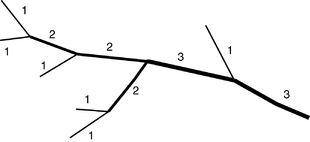
\includegraphics[scale=.75]{immagini/ordine_horton.png}
    \caption{Criterio di assegnazione dell'ordine ai segmenti del reticolo idrografico, secondo Horton-Strahler.}
  \label{ordine_horton}
\end{figure}
Avendo assegnato ad ogni tratto un certo valore numerico, è possibile conoscere la numerosità di ogni ordine. \\
Nel nostro caso, il reticolo idrografico del bacino è formato da un'asta principale e da quattro tratti laterali, disposti sulla destra idraulica di quella maggiore.\\
Essendo che il segmento coincidente con il punto di chiusura possiede valore 3, di conseguenza l'intero bacino idrologico è di ordine 3.\\
La frequenza degli ordini dei segmenti è la seguente:
\begin{table}[H] \centering
    \begin{tabular}{cc}
\toprule
    Ordine u & Segmenti Nu \\
\midrule    
    1        & 5           \\
    2        & 2           \\
    3        & 1           \\
\bottomrule    
\end{tabular}
\end{table}